\subsection{Performance Analysis of Algorithms}
\label{subsec:data process}

In the section \ref{sec:model}, we have introduced our algorithms for band adaptation. 
In this section, we investigate the performance for evaluation and compare the proposed schemes with the data collected in
\ref{subsec:ichannel} and \ref{subsec:insitu}.

To investigate the performance, \emph{Accuracy} and \emph{Throughput Gap} are used to represent the performance of band estimation.
\emph{Accuracy} is defined as the percentages of best band prediction matches the measured best band as formula \ref{equation:df accuracy}.


\begin{align}
\label{equation:df accuracy}
Accuracy = \frac{Correct\ Prediction\ Slots}{All\ Predict\ Time\ Slots}
\end{align}



\emph{Throughput Gap} is the deference between the performance of estimation throughput and measured best throughput as defiend in formula \ref{equation:df gap}.

\begin{align}
\label{equation:df gap}
Throughput\ Gap = \frac{\sum{Max\ Tpt- Estimate\ Band\ Tpt}}{\sum{Max\ Tpt}}
\end{align}

%Ideal channel based process and accuracy computation

For the \emph{SNR based Throughput Look up Algorithm}, the \emph{Accuracy} and \emph{Throughput Gap} can be calculated through all the prediction and measured data.
%ML and LB algorithms process and accuracy computation
For \emph{Machine Learning Algorithm} and \emph{Location Based Algorithm}, the data set is divided in to training set and testing set for evaluation.
%The \emph{Accuracy} performance is counted as the correct prediction of the test set as defined in \ref{equation:df accuracy}. 



\begin{figure}
\centering
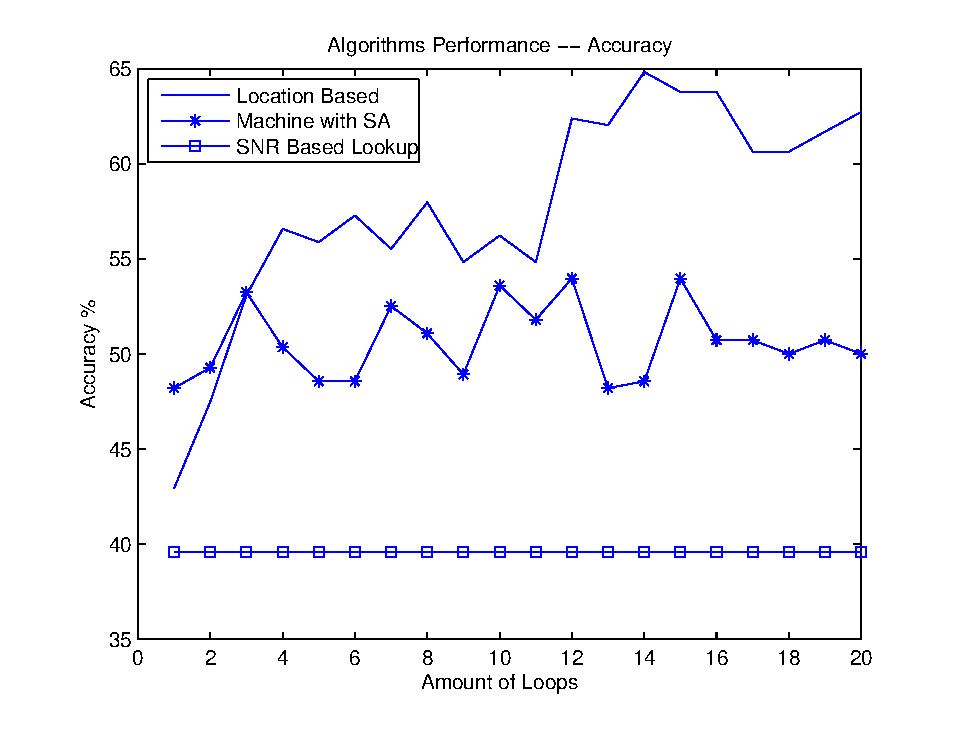
\includegraphics[width=85mm]{figure/performance}
\caption{Accuracy of 3 Algorithms}
\label{fig:performance}
\end{figure}

In figure \ref{fig:performance} we show the performance of the 3 algorithms. 
The x-axis in figure \ref{fig:performance} is the number of loops the mobile node traveled through the park. 
The flat curve with square represents the performance of \emph{SNR based Look up Algorithm}, it keeps as 39.2\% across all the data.
The curve with "*" represents the performance of \emph{Machine Learning Algorithm}. From the curve, we could see the accuracy of this algorithm is better than the \emph{SNR based Look up Algorithm}, but the accuracy is not directly related to the amount of training set. 
There are multiple dips on the curve. 
Because the relationship between the context information and the best band changing from loop to loop, additional training data would be treated as noisy data in the expanded training set for \emph{Machine Learning Algorithm}. It can increase the training set size, but it also introduce noise. When the pattern changed a lot, the accuracy can decrease.
The \emph{Location based Look up Algorithm} gets the highest accuracy as 65\% in figure \ref{fig:performance}. We could see the \emph{Accuracy} increase as the training data goes up through there is some dips on the curve. The in-situ data can not guarantee has the same performance distirbution even under the limitations. These reasons could bring the dips of the algorithms. 


\begin{figure}
\centering
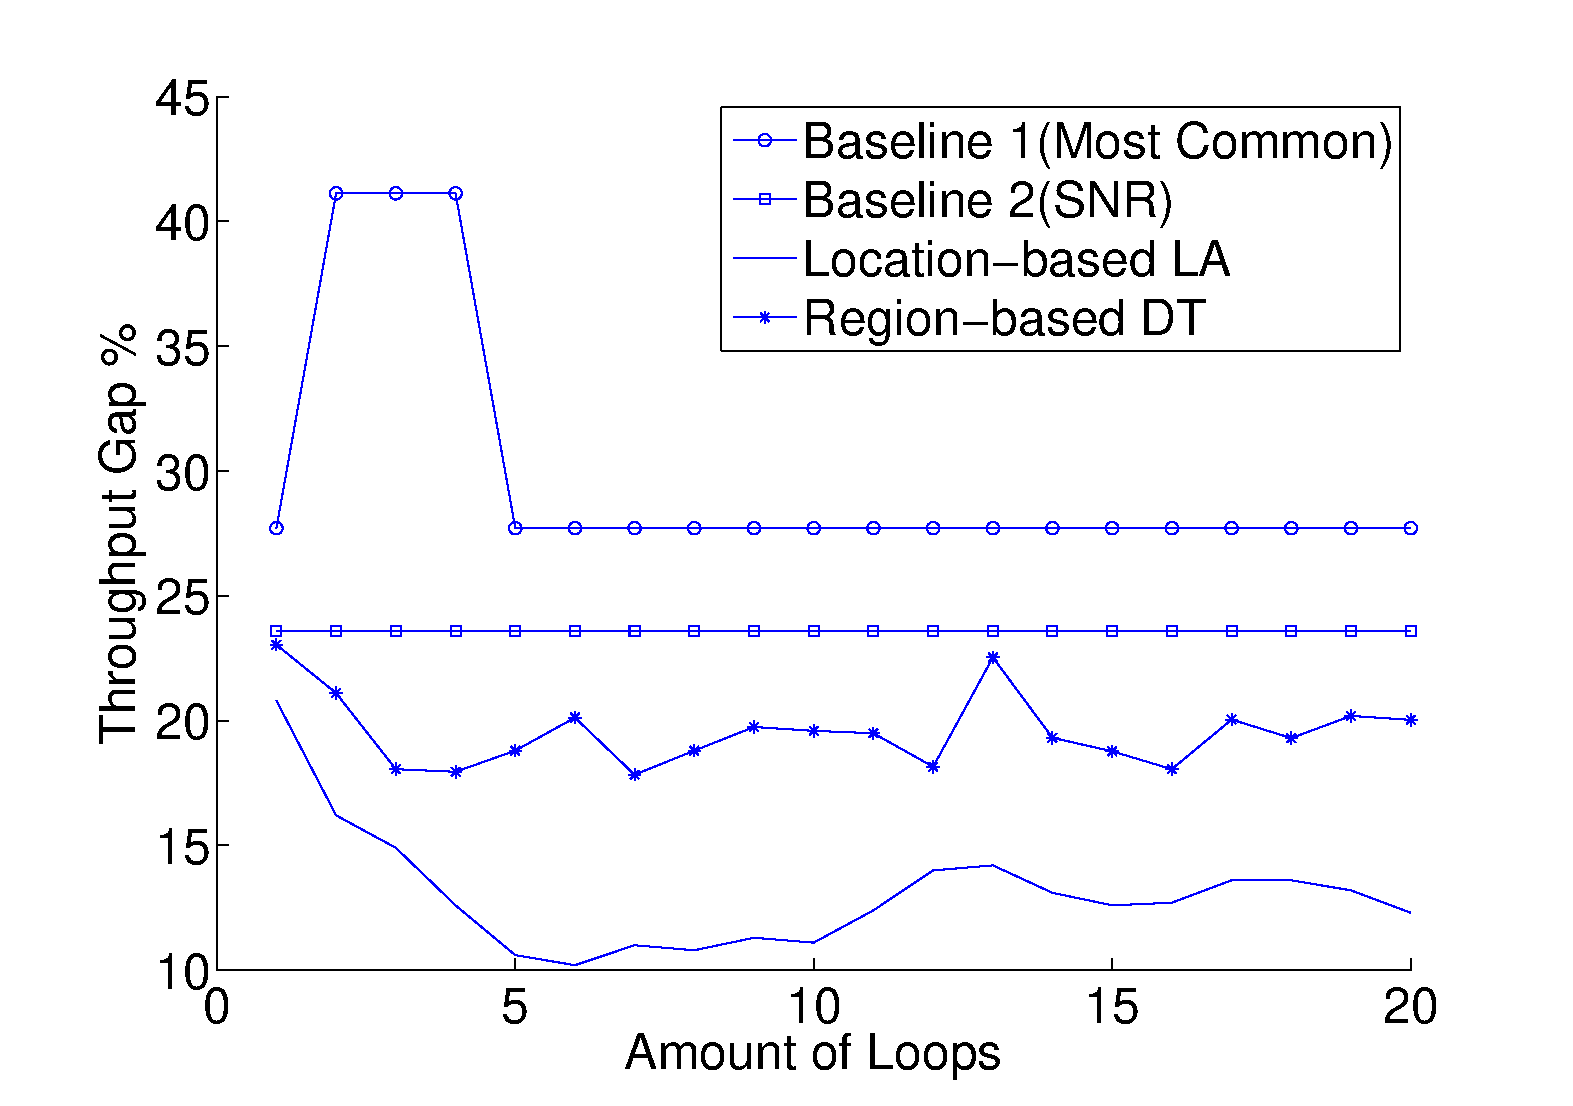
\includegraphics[width=85mm]{figure/performance_gap}
\caption{Throughput Gap of 3 Algorithms}
\label{fig:performance}
\end{figure}

In figure \ref{fig:performance_gap}, the \emph{Throughput Gap} of the 3 algorithms are investigated. \emph{SNR based Look up Algorithm} shows the gap upper bound in the figure. Both \emph{Machine Learning Algorithm} and \emph{Location based Look up Algorithm} have some gains as the training data increase in loops. Also, as explained in previous paragraph, the context information may change from loop to loop, time to time, this bring the dips on the two curves. 


In figure \ref{fig:region map}, the loop around the park is divided into 8 regions.

\begin{figure}
\centering
\includegraphics[width=85mm]{figure/region_map}
\caption{Split Regions}
\label{fig:region map}
\end{figure}

The \emph{Accuracy} performance of \emph{Location based Look up Algorithm} and \emph{Split Region Machine Learning Algorithm} in the same training set and testing set is shown in figure \ref{fig:mvsl}

 
\begin{figure}
\centering
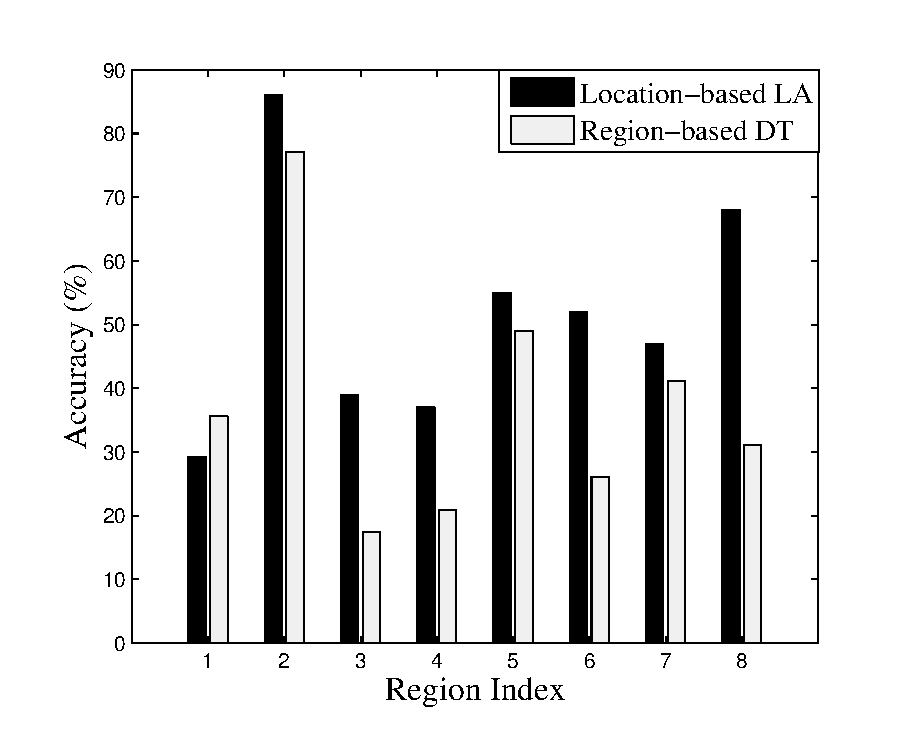
\includegraphics[width=85mm]{figure/mvsl}
\caption{Performance in Different Regions of Split Region Machine Learning Algorithm and Location Based Look up Algorithm}
\label{fig:mvsl}
\end{figure}

Only in Region 1, the \emph{Machine Learning Algorithm} has better accuracy than \emph{Location based Look up Algorithm}. \emph{Location based Look up Algorithm} has more limitation than \emph{Machine Learning Algorithm} and considering the data points at the boundary of each region. This makes the \emph{Location based Look up Algorithm} has a better accuracy.

We have investigated the performance of the algorithms in one experimental data set and shown the gains of them. Multi-band channels are complex system that knowing more information can make better decisions.



